
% \subsection{Cryptarithmetic Problem}
% Cryptarithm, mathematical recreation in which the goal is to decipher an arithmetic problem in which letters have been substituted for numerical digits.
% The term crypt-arithmetic was introduced in 1931, when a multiplication problem appeared in the Belgian journal Sphinx [Fig. 1]:
% \begin{figure}
% \centerline{
% 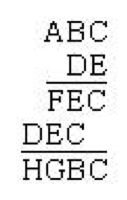
\includegraphics[width=0.15\textwidth]{fig/fig_crypt_1.png}}
% \caption{Cryptarithmetic Multiplication Problem}
% \label{fig:crypt_multi}
% \end{figure}

% Cryptarithm now denotes mathematical problems usually calling for addition, subtraction, multiplication, or division and replacement of the digits by letters of the alphabet or some other symbols.\footnote{\textit{Cryptarithm} is defined in \cite{BritannicaCrypt}.}

% The problem discussed here involves a simple addition of two terms consisting of characters resulting in a sum term. The goal is to map each character to a digit such that the summation of two numeric terms matches the character mapping of the sum term.
% Here are some of the constraints:
% \begin{itemize}
% \item Leading character for each term cannot be mapped to 0
% \item There should be no more than 10 distinct characters. For example, $abcde+efghi=ijklm$ has no solutions (there are 12 distinct characters)
% \item The summation should be the longest word. For example, $ab+cde=fg$ has no solutions ($cde$ is longer than $fg$)
% \item The summation cannot be too long. For example, $ab+cd=efgh$ has no solutions ($ab$ and $cd$ range from 10 to 99, so the summation cannot be more than 198).\footnote{These are mentioned as tips in \cite{CryptPuzzleSolver}.}
% \end{itemize}

% For example,
% \begin{figure}
% \centerline{
% 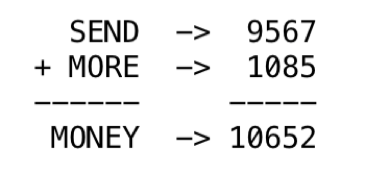
\includegraphics[width=0.5\textwidth]{fig/fig_crypt_2.png}}
% \caption{Cryptarithmetic Summation Problem}
% \label{fig:crypt_sum}
% \end{figure}

% Due to the nature of the problem, there might exist more than one solution to it. The goal is to find all such solutions.

% One way is to try to fill the columns from right to left, by assigning (unifying) valid digits to characters as we move to the left. In the beginning, the digit pool will have all 10 digits to choose from. Once we assign a digit to a character, we remove it from the digit pool. Doing this keeps us from picking the already assigned digit again for a different character (eliminating possibilities). When we reach the leftmost column and successfully assign a digit to the final character, we get the one possible solution to the problem.

% At any point during assignment (unification), if we come across an invalid choice, we will skip to the next available choice until we exhaust all the choices from the digit pool. In which case, we backtrack to the previous level, make a different choice and continue from there. This mimics the depth-first-search which is a core functionality of Prolog. To achieve the same in Python, we will make use of PyLog.

% First, we will set up the problem into a proper representation. 
% \begin{enumerate}
% \item Create a dictionary of a character to an uninstantiated PyValue for all unique characters
% \item Create 4 lists of PyValues for carries, term1, term2 and sum
% \item Length of each list would be the length of the sum term plus 1
% \item Pad all three terms with PyValue(0) and fill the remaining with uninstantiated PyValue instance from the dictionary
% \item Fill the carry list with unique uninstantiated PyValues
% \item Create a list leading\_digits that maintains all the PyValue instances that are at the beginning of any term. We use this to avoid unifying digit 0 to any of these PyValue.
% \end{enumerate}

% Here is how it will look like:
% \begin{figure}
% \centerline{
% 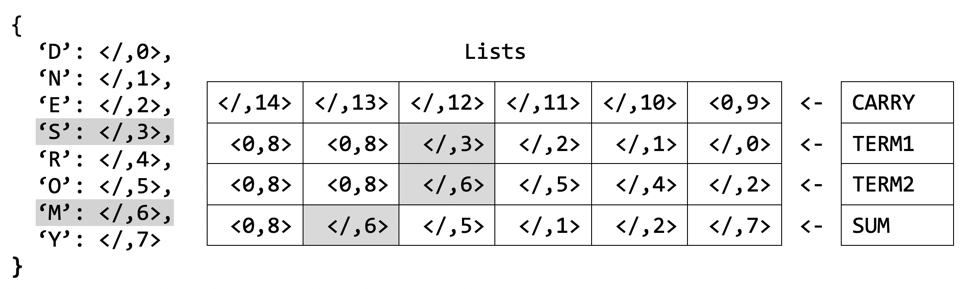
\includegraphics[width=\textwidth]{fig/fig_crypt_3.png}}
% \caption{Graphical Representation of the problem setup}
% \label{fig:crypt_setup}
% \end{figure}
 
% Here, each \pyth{<value, obj_id>} represents a PyValue object. As discussed above, each list contains a PyValue object. It can be seen that a character is represented by the same PyValue object across all 3 arrays (i.e. Term1, Term2 and Sum array). For example, ‘E’ appears in all 3 terms, and is represented by the same object \pyth{</,2>} in all 3 lists.

% Some of the fields are grayed out. These are the leading characters, and therefore cannot be assigned to a digit 0. We keep track of this by looking at leading\_digits list.

% Here is a code that achieves the above setup:

% \begin{python3}
% def set_up_puzzle(t1: str, t2: str, sum: str, _Z: PyValue) -> \
%                   Optional[Tuple[List[PyValue], List[PyValue], List[PyValue], List[PyValue], List[PyValue]]]:
%   """
%   Convert the initial string representation to (uninstantiated) PyValues.
%   t1 and t2 are the numbers to be added. sum is the sum.
%   _Z is PyValue(0). It will be replaced by leading blanks.
%   """
%   Var_Letters = sorted(list(set(t1 + t2 + sum)))
%   if len(Var_Letters) > 10:
%     print(f'Too many variables: {Var_Letters}')
%     return
%   Vars_Dict = {V: PyValue() for V in Var_Letters}
%   length = len(sum) + 1
%   T1 = (length - len(t1)) * [_Z] + letters_to_vars(t1, Vars_Dict)
%   T2 = (length - len(t2)) * [_Z] + letters_to_vars(t2, Vars_Dict)
%   Sum = (length - len(sum)) * [_Z] + letters_to_vars(sum, Vars_Dict)
%   # Leading_Digits are the variables that should not be assigned 0.
%   Leading_Digits = letters_to_vars({t1[0], t2[0], sum[0]}, Vars_Dict)
%   Carries = [PyValue() for _ in range(length - 1)] + [PyValue(0)]
%   return (Carries, T1, T2, Sum, Leading_Digits)
% \end{python3}
% \begin{lstlisting} [caption={cryptarithmetic\_set\_up\_puzzle},  label={lis:cryptarithmetic}]
% \end{lstlisting}

% Now that we have a setup, we can start solving the puzzle. To solve the puzzle, all we need is the parameters Carries, T1, T2, Sum, and Leading\_Digits created above. If it finds a valid solution, it yields at that point. We capture this yield, which acts like a halt in the execution of a function and prints out the state of all the PyValue objects to the console. This is one solution to the puzzle. We can iterate through this generator function until exhaustion to find out all possible solutions to the puzzle. Here is a code that iterates through the solve() generator function.

% \begin{python3}
% def solve_crypto(t1: str, t2: str, sum: str):
%   _Z = PyValue(0)
%   (Carries, T1, T2, Sum, Leading_Digits) = set_up_puzzle(t1, t2, sum, _Z)
%   want_more = None
%   Blank = PyValue(' ')
%   for _ in solve(Carries, T1, T2, Sum, Leading_Digits):
%     # We have a solution.
%     # Replace the leading _Z zeros with blanks and convert each number to a string.
%     # We can discard T1[0], T2[0], and Sum[0] because we know they will be 0.
%     (t1_out, t2_out, tot_out) = (solution_to_string(T, _Z, Blank) for T in [T1[1:], T2[1:], Sum[1:]])
%     print()
%     print(f'  {t1}  -> {t1_out}')
%     print(f'+ {t2}  -> {t2_out}')
%     print(f'{"-" * (len(sum)+1)}     {"-" * len(sum)}')
%     print(f' {sum}  -> {tot_out}')
%     ans = input('\nLook for more solutions? (y/n) > ').lower( )
%     want_more = ans[0] if len(ans) > 0 else 'n'
%     if want_more != 'y':
%       break
%   if want_more == 'y':
%     print('No more solutions.')

% \end{python3}
% \begin{lstlisting} [caption={cryptarithmetic\_solve\_crypto},  label={}]
% \end{lstlisting}

% Let’s talk about how the solve() function solves the puzzle. It starts filling columns from right to left. fill\_column() takes the list of PyValue objects of a column and list of all the available digits to choose from as input. Once it completes filling a column, it yields back the remaining digits in the form of a list. These remaining digits are then passed on to the next fill\_column() call to fill the next column. Once the last column is filled successfully, it halts the execution of solve() by yield statement.

% fill\_column() works in a recursive manner. It iterates through all the available digits from the pool and assigns (unifies) the digit to the first PyValue from the input list, and recursively calls itself for the remaining PyValues and digit pool. Once all the PyValues are assigned (i.e. PVs == False), it performs the validation of the current choices. It sums up the values of terms’ PyValues along with the carry at the current index, finds the mod of 10, and matches it to the expected sum digit to the current index. If this holds, meaning current choices are correct for the column, it assigns (unifies) the remaining carry value to the next index’s carry. These operations are taken care of by a method complete\_column().

% Once the last column is filled, to check if the solution is valid or not, it performs the last check where it ensures there is no leftover carry stored in the first object of the carry list.

% It very crucial that, while unifying any PyValue with a digit, we need to first ensure that it is uninstantiated i.e. it has not been unified with any digit yet. A PyValue object has a method is\_instantiated() which returns a Boolean that tells if the object is already unified or not.

% One more important point to take note is the constraint that any leading character cannot be unified with a digit 0. We ensure this by putting the check \pyth{if not (digits_in[i] == 0 and PV in Leading_Digits)} while choosing a digit for the current PyValue instance.

% The following is the code that achieves the above solution.

% \begin{python3}
% def solve(Carries: List[PyValue],
%           Term1: List[PyValue],
%           Term2: List[PyValue],
%           Sum: List[PyValue],
%           Leading_Digits: List[PyValue]):
%   """
%   Solve the problem.
%   The two embedded functions below refer to the lists in solve's params.
%   The lists never change, but their elements are unified with values.
%   No point is copying the lists repeatedly. So embed the functions that refer to them.
%   """

%   def fill_column(PVs: List[PyValue], index: int, digits_in: List[int]):
%     """
%     PVs are the digits in the current column to be added together, one from each term.
%     digits-in are the digits that have not yet been assigned to a Var.
%     Find digits in digits_in that make the column add up properly.
%     Return (through yield) the digits that are not yet used after the new assignments.
%     We do this recursively on PVs--even though we are currently assuming only two terms.
%     """
%     if not PVs:
%       # We have instantiated the digits to be added.
%       # Instantiate Sum_Dig (if possible) and Carries[index - 1] to the total.
%       # Completing the column is a bit more work than it might seem.
%       (carry_in, digit_1, digit_2) = (D.get_py_value( ) for D in [Carries[index], Term1[index], Term2[index]])
%       total = sum([carry_in, digit_1, digit_2])
%       (carry_out, sum_dig) = divmod(total, 10)
%       yield from complete_column(carry_out, Carries[index-1], sum_dig, Sum[index], digits_in, Leading_Digits)

%     else:
%       # Get head and tail of PVs.
%       [PV, *PVs] = PVs
%       # If PV already has a value, nothing to do. Go on to the remaining PVs.
%       if PV.is_instantiated( ):
%         yield from fill_column(PVs, index, digits_in)
%       else:
%         # Give PV one of the available digits. Through "backup" all digits will be tried.
%         for i in range(len(digits_in)):
%           if not (digits_in[i] == 0 and PV in Leading_Digits):
%             for _ in unify(PV, digits_in[i]):
%               yield from fill_column(PVs, index, digits_in[:i] + digits_in[i + 1:])

%   def solve_aux(index: int, digits_in: List[int]):
%     """ Traditional addition: work from right to left. """
%     # When we reach 0, we're done.
%     if index == 0:
%       # Can't allow a carry to this position.
%       if Carries[0].get_py_value() == 0:
%         yield
%       else:
%         # If we reach index == 0 but have a carry into the last column, fail.
%         # Won't have such a carry with only two terms. But it might happen with many terms,.
%         return
%     else:
%       for digits_out in fill_column([Term1[index], Term2[index]], index, digits_in):
%           yield from solve_aux(index-1, digits_out)
    
%   yield from solve_aux(len(Carries)-1, list(range(10)))


% def complete_column(carry_out: int, Carry_Out_Dig: PyValue,
%                     sum_dig: int, Sum_Dig: PyValue,
%                     digits_in: List[int], Leading_Digits):
%   """
%   If Sum_Dig (the variable representing the digit in the sum for this column) is not yet instantiated,
%   instantiate it to sum_dig  (if that digit is available). If Sum_Dig is already instantiated, ensure
%   it is consistent with the sum_dig. Instantiate Carry_Out_Dig to carry_out.
%   """
%   # Is Sum_Dig uninstantiated? If so, instantiate it to sum_digit if possible.
%   # Then instantiate Carry_Out_Dig, and return (yield) digits_in with sum_digit removed.
%   if not Sum_Dig.is_instantiated():
%     if sum_dig not in digits_in:
%       # sum_dig is not available in digits_in. Fail, i.e., return instead of yield.
%       return

%     # sum_dig is available in digits_in. Give it to Sum_Dig as long as this does not give
%     # 0 to one of the leading digits.
%     if not (sum_dig == 0 and Sum_Dig in Leading_Digits):
%       for _ in unify_pairs([(Carry_Out_Dig, carry_out), (Sum_Dig, sum_dig)]):
%         # Remove sum_digit from digits_in
%         i = digits_in.index(sum_dig)
%         yield digits_in[:i] + digits_in[i + 1:]

%   # If Sum_Dig is instantiated, is it equal to sum_digit?
%   # If so, instantiate Carry_Out_Dig and return the current digits_in.
%   elif sum_dig == Sum_Dig.get_py_value( ):
%     for _ in unify(Carry_Out_Dig, carry_out):
%       yield digits_in
% \end{python3}
% \begin{lstlisting} [caption={cryptarithmetic\_solve},  label={}]
% \end{lstlisting}
